\section{Практическая часть}

Для написания програмы основным языком был выбран Java, поскольку в данном курсе мы параллельно изучаем этот язык и написание данной программы
является хорошей практикой для его изучения.

\subsection{Как пользоваться программой}

Запускаем jar-файл с параметром '-h', чтобы вызвать меню помощи:
\begin{figure}[h!]
  \center{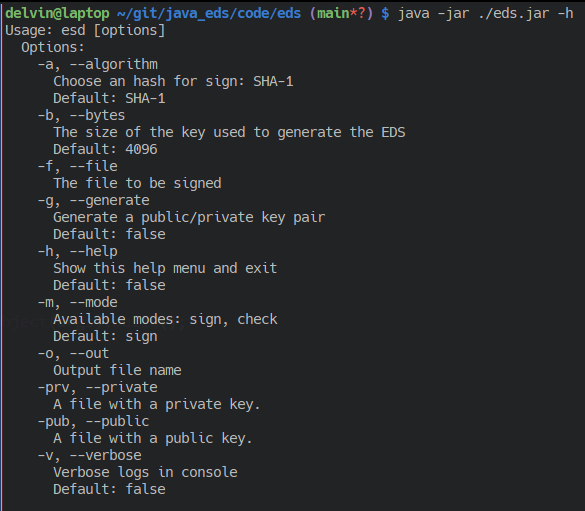
\includegraphics[scale=0.9]{img/program_usage}}
  \caption{Меню помощи}
\end{figure}

\subsubsection{Алгоритм}
Ключ '-a' отвечает за алгоритм хэш-функции. Программа написана с использованием интерфейсов, чтобы максимально упростить задачу добавления новых хэш-функций.
Как видно из рисунка выше, для данной работы был реализован только SHA-1, который является опцией по-умолчанию, поэтому этот параметр можно не указывать.

\subsubsection{Размер ключа}
Ключ '-b' отвечает за размер модуля, который будет генерироваться для алгоритма RSA.

\subsubsection{Генерация ключей}
Ключ '-g' отвечает за генерацию открытого и закрытого ключей ЭЦП.

\subsubsection{Файлы}
Ключ '-f' отвечает за файл, который необходимо подписать. Ключ '-o' - за файл, куда записать данные.

\subsubsection{Режимы работы}
Ключ '-m' отвечает за режим работы программы. По-умолчанию программа будет подписывать файл, если нам необходимо проверить подпись, то нужно передать параметр 'check'.

\subsubsection{Чтение ключей из файлов}
Ключ '-prv' указывает откуда читать данные для приватного ключа.

Ключ '-pub' указывает откуда читать данные для публичного ключа.

\subsubsection{Подробный режим}
Ключ '-v' говорит программе, что необходимо подробно описывать ход своей работы.

\newpage
\subsection{Примеры использования программы}

\begin{figure}[h!]
  \center{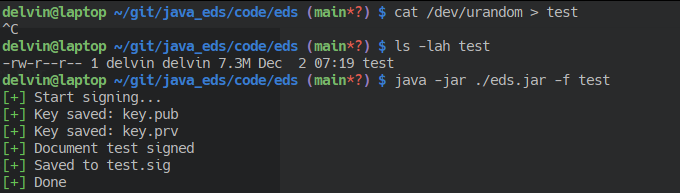
\includegraphics[scale=0.9]{img/simple_sign.png}}
  \caption{Подпись файла}
\end{figure}

\begin{figure}[h!]
  \center{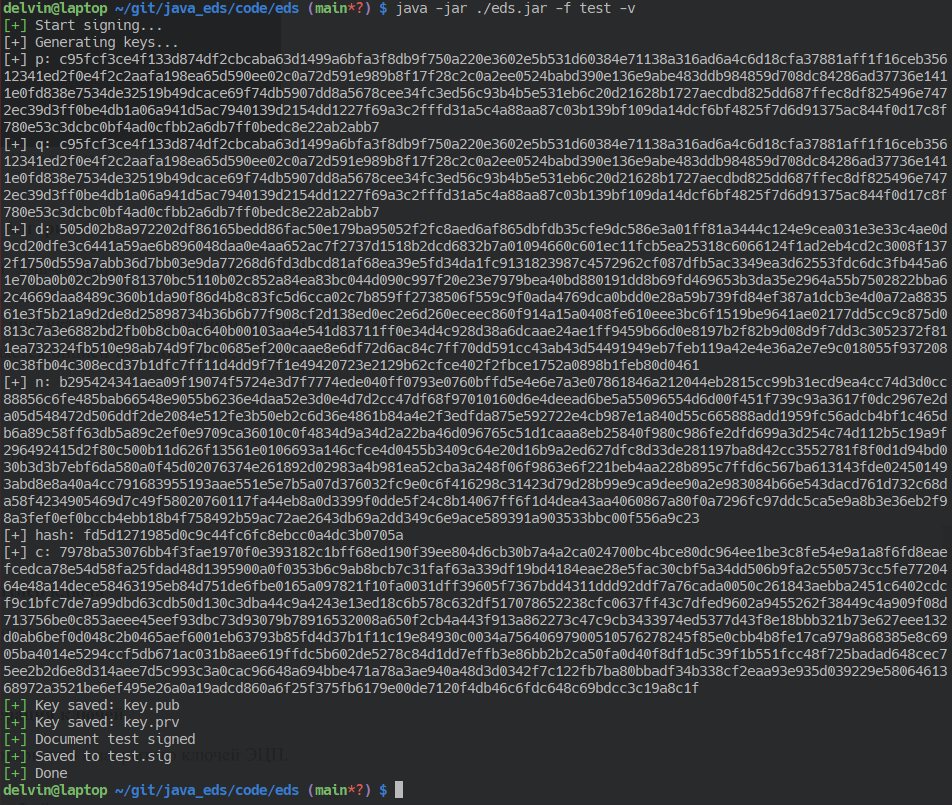
\includegraphics[scale=0.7]{img/simple_sign_verbose.png}}
  \caption{Подпись файла в подробном режиме}
\end{figure}

Как можно видеть на рисунках выше, создаётся два файла с публичным и приватным ключом. Помимо этого, в файл записывается определенная структура, которая говорит, что документ был подписан. О ней читатель узнает позже.

\begin{figure}[h!]
  \center{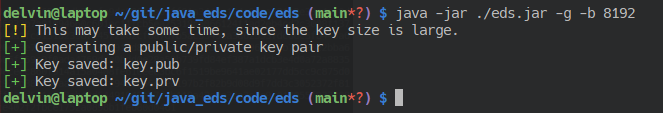
\includegraphics[scale=0.8]{img/key_gen.png}}
  \caption{Генерация ключей}
\end{figure}

\begin{figure}[h!]
  \center{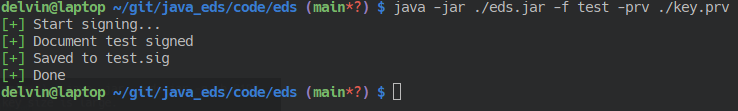
\includegraphics[scale=0.8]{img/use_key_sign.png}}
  \caption{Использование сгенерированных ключей для подписи}
\end{figure}

\begin{figure}[h!]
  \center{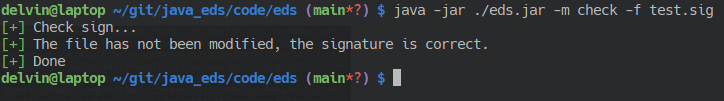
\includegraphics[scale=0.8]{img/base_check_sign.png}}
  \caption{<<Честная>> проверка подписи}
\end{figure}